%
%  Chris Thoma
%
\documentclass[12pt,fullpage]{article}
\usepackage{fullpage}
\usepackage{psfrag}                                          % LaTeX graphics tool
\usepackage{pslatex}                                         % avoids the default cmr font
\usepackage{graphicx}                                        % graphics package 
\usepackage{epsfig} 
\usepackage{hyperref}
\usepackage{color}

\begin{document}

\noindent
{\bf Triangular distribution} (from \color{blue}\url{http://www.math.wm.edu/~leemis/chart/UDR/UDR.html}\color{black})

\noindent
The shorthand $X \sim {\rm triangular}(a, m, b)$ is used to indicate that the
random variable $X$ has the triangular distribution with parameters $a$, $m$ and $b$.
A triangular random variable $X$ has probability density function 
$$
f(x) = \left\{ \begin{array}{ll}
		\frac{2 (x - a)}{(b - a) (m - a)} & \qquad a < x < m \\ [0.05in]
		\frac{2 (b - x)}{(b - a) (b - m)} & \qquad m \leq x < b.
		\end{array} \right. \, 
$$		
The triangular distribution can be used as an approximate model when there are no data values.
An expert familiar with the population specifies a minium value $a$, a most likely value $m$,
and a maximum value $b$.
The probability density function is illustrated below.
{\begin{figure}[h!]
\begin{center}
\psfrag{labx}{$x$}
\psfrag{labf}{$f(x)$}
\psfrag{laba}{$a$}
\psfrag{labm}{$m$}
\psfrag{labb}{$b$}
\includegraphics[width=3.2in]{TriangularPlot.ps}
\end{center}
\end{figure}}

\noindent
The cumulative distribution function on
the support of $X$ is 
$$
F(x) = P(X \le x) = \left\{ \begin{array}{ll}
		\frac{(x - a) ^ 2}{(b - a) (m - a)} & \qquad a < x < m \\ [0.05in]
		1 - \frac{(b - x) ^ 2}{(b - a) (b - m)} & \qquad m \leq x < b.
		\end{array} \right. \, 
$$
The survivor function on the support of $X$ is
$$
S(x) = P(X \ge x) = \left\{ \begin{array}{ll}
		1 - \frac{(x - a) ^ 2}{(b - a) (m - a)} & \qquad a < x < m\\ [0.05in]
		\frac{(b - x) ^ 2}{(b - a) (b - m)} & \qquad m \leq x < b.
		\end{array} \right. \, 
$$
The hazard function on the support of $X$ is
$$
h(x) = \frac{f(x)}{S(x)} = \left\{ \begin{array}{ll}
		\frac{2 (a - x)}{ab - mb + ma + x ^ 2 - 2 ax} & \qquad a < x < m \\ [0.05in]
		\frac{2}{b - x} & \qquad m \leq x < b.
		\end{array} \right. \, 
$$
The moment generating function of $X$ is
$$
M(t) = E\left[ e ^ {tX} \right] = -\frac{2 (- m e ^ {ta} + b e ^ {ta} + b e ^ {tm} + a e ^ {tm} - a e ^ {tb} + m e ^ {tb})} {(a - m) (a - b) (m - b) t ^2} \qquad \qquad  t > 0.
$$
The characteristic function of $X$ is
$$
\phi(t) = E\left[ e ^ {it X} \right] = \frac{2(- m e ^ {it a} + b e ^ {it a} + b e ^ {it m} + a e ^ {it m} - a e ^ {it b} + m e ^ {it b})} {(a - m) (a - b) (m - b)t ^ 2} \qquad \qquad  t > 0.
$$
The population mean, variance, skewness, and kurtosis of $X$ are
$$
E[X] = \frac{a + m + b} {3} \quad \quad 
V[X] = \frac{a ^ 2 + m ^ 2 + b ^ 2 - ab - am - mb} {18} \quad \quad 
$$
$$
E\left[ \left( \frac{X - \mu}{\sigma} \right) ^ 3 \right] =  \frac{\sqrt{2}(a + b - 2m) (2a - b - m) (a - 2b + m)} {5 (a ^ 2 + b ^ 2 + m ^ 2 - ab - am - bm) ^ {3/2}}\quad \quad
E\left[ \left( \frac{X - \mu}{\sigma} \right) ^ 4 \right] = \frac{12}{5}.
$$
%\newpage
\noindent
{\bf APPL verification:}
The APPL statements
\begin{verbatim}
X := TriangularRV(a, m, b);
CDF(X);
SF(X);
HF(X); 
Mean(X);
Variance(X);
Skewness(X);
Kurtosis(X);
MGF(X);
\end{verbatim}
verify the cumulative distribution function, survivor function, hazard function, population mean, variance, skewness, kurtosis, and moment generating function.

\end{document}
